\documentclass[10pt,twocolumn,letterpaper]{article}

\usepackage{cvpr}
\usepackage{times}
\usepackage{epsfig}
\usepackage{graphicx}
\usepackage{amsmath}
\usepackage{amssymb}
\usepackage{tikz}
\usepackage{pgfplots}
\usetikzlibrary{shadows,trees}

\usepackage{verbatim}
\usepackage{bm}
\usepackage{microtype}
\usepackage{url}
\usepackage{multirow}
\usepackage{subcaption}
\usepackage{booktabs} % for better tables

\newlength{\eqs}
\setlength{\eqs}{-0.04in}

\usepackage{enumitem}
\setitemize[0]{leftmargin=15pt}

\newenvironment{tight_itemize}{
\begin{itemize}[leftmargin=10pt]
  \setlength{\topsep}{0pt}
  \setlength{\itemsep}{0pt}
  \setlength{\parskip}{0pt}
  \setlength{\parsep}{0pt}
}{\end{itemize}}



% If you comment hyperref and then uncomment it, you should delete
% egpaper.aux before re-running latex.  (Or just hit 'q' on the first latex
% run, let it finish, and you should be clear).
\usepackage[pagebackref=true,breaklinks=true,letterpaper=true,colorlinks,bookmarks=false]{hyperref}


% New math commands/abreviations

\newcommand{\bA}{\mathbf{A}}
\newcommand{\bB}{\mathbf{B}}
\newcommand{\bC}{\mathbf{C}}
\newcommand{\bD}{\mathbf{D}}
\newcommand{\bE}{\mathbf{E}}
\newcommand{\bF}{\mathbf{F}}
\newcommand{\bG}{\mathbf{G}}
\newcommand{\bH}{\mathbf{H}}
\newcommand{\bI}{\mathbf{I}}
\newcommand{\bJ}{\mathbf{J}}
\newcommand{\bK}{\mathbf{K}}
\newcommand{\bL}{\mathbf{L}}
\newcommand{\bM}{\mathbf{M}}
\newcommand{\bN}{\mathbf{N}}
\newcommand{\bO}{\mathbf{O}}
\newcommand{\bP}{\mathbf{P}}
\newcommand{\bQ}{\mathbf{Q}}
\newcommand{\bR}{\mathbf{R}}
\newcommand{\bS}{\mathbf{S}}
\newcommand{\bT}{\mathbf{T}}
\newcommand{\bU}{\mathbf{U}}
\newcommand{\bV}{\mathbf{V}}
\newcommand{\bW}{\mathbf{W}}
\newcommand{\bX}{\mathbf{X}}
\newcommand{\bY}{\mathbf{Y}}
\newcommand{\bZ}{\mathbf{Z}}

\newcommand{\ba}{\mathbf{a}}
%\newcommand{\bb}{\mathbf{b}}
\newcommand{\bc}{\mathbf{c}}
\newcommand{\bd}{\mathbf{d}}
\newcommand{\be}{\mathbf{e}}
%\newcommand{\bf}{\mathbf{f}}
\newcommand{\bg}{\mathbf{g}}
\newcommand{\bh}{\mathbf{h}}
\newcommand{\bi}{\mathbf{i}}
\newcommand{\bj}{\mathbf{j}}
\newcommand{\bk}{\mathbf{k}}
\newcommand{\bl}{\mathbf{l}}
%\newcommand{\bm}{\mathbf{m}}
\newcommand{\bn}{\mathbf{n}}
%\newcommand{\bo}{\mathbf{o}}
\newcommand{\bp}{\mathbf{p}}
\newcommand{\bq}{\mathbf{q}}
\newcommand{\br}{\mathbf{r}}
\newcommand{\bs}{\mathbf{s}}
\newcommand{\bt}{\mathbf{t}}
\newcommand{\bu}{\mathbf{u}}
\newcommand{\bv}{\mathbf{v}}
\newcommand{\bw}{\mathbf{w}}
\newcommand{\bx}{\mathbf{x}}
\newcommand{\by}{\mathbf{y}}
\newcommand{\bz}{\mathbf{z}}

\newcommand{\bff}{\mathbf{f}}

\newcommand{\bo}{\mathbf{0}}
\newcommand{\tx}{\tilde{\mathbf{x}}}


\newcommand{\hbn}{{\widehat{\mathbf{n}}}}
\newcommand{\hbs}{{\widehat{\mathbf{s}}}}
\newcommand{\hbh}{{\widehat{\mathbf{h}}}}
\newcommand{\hbv}{{\widehat{\mathbf{v}}}}
\newcommand{\hbw}{{\widehat{\mathbf{w}}}}
\newcommand{\hbc}{{\widehat{\mathbf{c}}}}

\newcommand{\hh}{{\widehat{h}}}
\newcommand{\hn}{{\widehat{n}}}
\newcommand{\hx}{{\widehat{x}}}
\newcommand{\hy}{{\widehat{y}}}
\newcommand{\hz}{{\widehat{z}}}


% Mathcal definitions
\newcommand{\cS}{\mathcal{S}}
\newcommand{\cD}{\mathcal{D}}
\newcommand{\cP}{{\mathcal{P}}}
\newcommand{\cU}{{\mathcal{U}}}
\newcommand{\cV}{{\mathcal{V}}}
\newcommand{\cE}{{\mathcal{E}}}
\newcommand{\cQ}{{\mathcal{Q}}}
\newcommand{\cG}{{\mathcal{G}}}
\newcommand{\cB}{{\mathcal{B}}}
\newcommand{\cI}{\mathcal{I}}
\newcommand{\cL}{\mathcal{L}}
\newcommand{\cR}{{\mathcal{R}}}
\newcommand{\cC}{{\mathcal{C}}}
\newcommand{\cO}{{\mathcal{O}}}
\newcommand{\cX}{{\mathcal{X}}}



% Mathbb definitions
\newcommand{\bbp}{\mathbb{P}}
\newcommand{\bbP}{\mathbb{P}}
\newcommand{\bbQ}{\mathbb{Q}}
\newcommand{\bbr}{\mathbb{R}}
\newcommand{\bbR}{\mathbb{R}}
\newcommand{\bbS}{\mathbb{S}}
\newcommand{\bbN}{\mathbb{N}}



% Mathbm definitions
\newcommand{\balpha}{{\bm{\alpha}}}
\newcommand{\bbeta}{{\bm{\beta}}}
\newcommand{\bgamma}{{\bm{\gamma}}}
\newcommand{\bepsilon}{{\bm{\epsilon}}}
\newcommand{\bmu}{{\bm{\mu}}}
\newcommand{\bpi}{\bm{\pi}}
\newcommand{\brho}{\bm{\rho}}
\newcommand{\bomega}{\bm{\omega}}
\newcommand{\bOmega}{\bm{\Omega}}
\newcommand{\bSigma}{\bm{\Sigma}}
\newcommand{\bGamma}{\bm{\Gamma}}



\newcommand{\id}{\mathbf{I}}
\newcommand{\tid}{\tilde{\id}}
\newcommand{\st}{{\textrm{subject to }}}


\newcommand{\bpm}{{\widehat{\bP}}}
\newcommand{\bxm}{{\widehat{\mathbf{X}}}}
\newcommand{\winf}{{{\bm{\Omega}}_\infty}}
%\newcommand{\bw}{{{\bm{\omega}}^*}}
\newcommand{\bwi}{{{\bm{\omega}}_i^*}}
\newcommand{\bwone}{{{\bm{\omega}}_1^*}}
\newcommand{\diac}{{{\bm{\omega}}^*}}
\newcommand{\iac}{{{\bm{\omega}}}}
\newcommand{\ac}{{{\bm{\Omega}}_\infty}}
\newcommand{\diaci}{{{\bm{\omega}}_i^*}}
\newcommand{\diacone}{{{\bm{\omega}}_1^*}}
\newcommand{\w}{{{\bm{\omega}}^*}}
\newcommand{\daq}{{\mathbf{Q}}_\infty^*}
\newcommand{\adq}{{\mathbf{Q}}_\infty^*}
\newcommand{\pinf}{{\bm{\pi}}_\infty}
\newcommand{\hinf}{{{\bH}_\infty}}
\newcommand{\hinft}{{{\bH}^\top_\infty}}
\newcommand{\hinfi}{{{\bH}^i_\infty}}
\newcommand{\hinfit}{{{\bH}^{i\top}_\infty}}
\newcommand{\hinfj}{{{\bH}^j_\infty}}
\newcommand{\hinfjt}{{{\bH}^{j\top}_\infty}}
\newcommand{\intval}[2]{[\, #1, #2 \, ]}
\newcommand{\camo}{\left[ \: \id \: \vert \: \bo \: \right]}
\newcommand{\cama}{\left[ \: \bA \: \vert \: \ba \: \right]}
\newcommand{\camr}{\left[ \: \bR \: \vert \: \bt \: \right]}
\newcommand{\camai}{\left[ \: \bA_i \: \vert \: \ba_i \: \right]}
\newcommand{\camri}{\left[ \: \bR_i \: \vert \: \bt_i \: \right]}

%\newcommand{\algorithmiccomment}[1]{//#1}
\newcommand{\lb}{\operatorname{\bf{Bound}}}
\newcommand{\branch}{\operatorname{\bf{Branch}}}
\newcommand{\feasible}{\operatorname{\bf{Feasible}}}
\newcommand{\trace}{\operatorname{Tr}}
\newcommand{\convenv}{\operatorname{\bf{convenv}}}
\newcommand{\rectangle}{Q}

\newcommand{\epi}{\operatorname{\bf{epi}}}
\newcommand{\dom}{\operatorname{\bf{dom}}}

\newcommand{\ophi}{f}
\newcommand{\phimin}{\ophi_{\text{min}}}
\newcommand{\philb}{\ophi_{\text{lb}}}
\newcommand{\phiub}{\ophi_{\text{ub}}}

\newcommand{\cvx}{{\mathrm{convex\_env}}}
\newcommand{\ccv}{{\mathrm{concave\_env}}}

\newcommand{\conc}[1]{\operatorname{conc}{#1}}
\newcommand{\conv}[1]{\operatorname{conv}{#1}}

%\newcommand{\deg}[1]{\operatorname{deg}{#1}}

\newcommand{\lmi}[1]{\operatorname{LMI}{#1}}

\newcommand{\fa}{\alpha}
\newcommand{\fb}{\beta}
\newcommand{\fc}{\gamma}


%\newcommand{\tr}{^\top}

\newcommand{\xlt}{x_l^{1/3}}
\newcommand{\xut}{x_u^{1/3}}
\newcommand{\tlt}{t_l^{1/3}}
\newcommand{\tut}{t_u^{1/3}}
\newcommand{\xl}{x_l}
\newcommand{\xu}{x_u}
\newcommand{\yl}{y_l}
\newcommand{\yu}{y_u}
\newcommand{\tl}{t_l}
\newcommand{\tu}{t_u}
\newcommand{\yp}{y_p}
\newcommand{\ypd}{y'_p}
\newcommand{\tp}{t_p}
\newcommand{\fl}{\frac{x - \xl}{\xu - \xl}}
\newcommand{\fu}{\frac{\xu - x}{\xu - \xl}}


% Bilinear definitions
\newcommand{\cl}{{\psi}^l}
\newcommand{\cu}{{\psi}^u}
\newcommand{\rect}{Q}
\newcommand{\cond}[1]{\operatorname{{\mathcal{C}}}{#1}}
\newcommand{\vol}[1]{\operatorname{vol}{#1}}

%\newcommand{\phimin}[1]{\operatorname{\Phi_{\textrm{min}}}{#1}}
%\newcommand{\philb}[1]{\operatorname{\Phi_{\textrm{lb}}}{#1}}
%\newcommand{\phiub}[1]{\operatorname{\Phi_{\textrm{ub}}}{#1}}


%\newcommand{\rank}{{\mathbf{rank}}}
%\newcommand{\diag}{{\mathrm{diag}}}

\newcommand{\rank}[1]{\operatorname{rank}{#1}}

%\newcommand{\bx}{x} %general unknown x
%\newcommand{\bX}{X} %scene point

\newcommand{\ix}{\bx} %image point
\newcommand{\ixa}{u} %1st coordinate of image point
\newcommand{\ixb}{v} %2nd coordinate of image point
\newcommand{\bXa}{U} %1st coordinate of scene point
\newcommand{\bXb}{V} %2nd coordinate of scene point
\newcommand{\bXc}{W} %3rd coordinate of scene point

\newcommand{\tr}{^\top}

\newcommand{\Linf}{L_{\infty}}
\newcommand{\Ltwo}{L_{2}}
\newcommand{\Lone}{L_{1}}
\newcommand{\Lp}{L_{p}}
\newcommand{\Lq}{L_{q}}

\def\smallmat#1{\left[\begin{smallmatrix}#1\end{smallmatrix}\right]}



\newcommand{\brs}{\bR_0}
\newcommand{\bts}{\bt_0}
\newcommand{\bzero}{\mathbf{0}}
\newcommand{\bdx}{\mathbf{dx}}

\newcommand{\p}{\partial}


\newcommand{\del}[1]{\nabla_{#1}}
\newcommand{\I}{\mathbf{I}}
\newcommand{\II}{\mathbf{II}}
\newcommand{\skewsymm}[1]{[{#1}]_\times}





% 3D pose of the cars and ego motion
\newcommand{\pos}[2]{\mathbf{p}^{#1}({#2})}
\newcommand{\ori}[2]{\mathbf{\omega}^{#1}(#2)}
\newcommand{\state}[2]{\mathbf{s}^{#1}(#2)}

% ego pose
\newcommand{\egop}[1][t]{\pos{c}{#1}}
\newcommand{\egoo}[1][t]{\ori{c}{#1}}
\newcommand{\egos}[1][t]{\state{c}{#1}}

% relative pose between camera and car $i$
\newcommand{\relp}[2]{\Omega^{#1}(#2)}
\newcommand{\relpz}[2]{\Omega_z^{#1}(#2)}

% 3D tracks on car $i$ in its own coordinate frame
\newcommand{\tracklets}{\mathbf{X}^{i}_o}
\newcommand{\tracklet}[1]{\mathbf{x}^{i}_{#1}}
% track projections on camera
\newcommand{\trackpit}[2]{\mathbf{u}_{#1}(#2)}
\newcommand{\trackp}[1]{\mathbf{u}_j(#1)}
\newcommand{\trackpj}[1]{\mathbf{u}_j(#1)}
% Unclassified track point projected on camera
\newcommand{\ucTrackp}{\mathbf{u}(t)}


% dimensions of car $i$
\newcommand{\dimsn}[1]{\mathbf{B}^{#1}}
\newcommand{\expDimsn}{\hat{\mathbf{B}}}

% projection function
\newcommand{\projectionOf}[1]{\pi_{\relp{i}{t}}\left(#1\right)}
\newcommand{\projectionOft}[1]{\pi_{\relp{i}{t+1}}\left(#1\right)}
\newcommand{\centerProj}{\bar{\pi}_{\relp{i}{t}}(\dimsn{i})}
\newcommand{\cornerProj}[1]{\pi^{#1}_{\relp{i}{t}}(\dimsn{i})}
\newcommand{\triangleProj}[1]{\triangle^{#1}_{\relp{i}{t}}(\dimsn{i})}

% bounding box corners on image
\newcommand{\bbt}[2]{\mathbf{d}^{#1}({#2})}
\newcommand{\bb}[1]{\mathbf{d}^{#1}(t)}


\newcommand{\Energy}[1]{\mathcal{E}^{it}_{\text{#1}}}
\newcommand{\pEnergy}[1]{\mathcal{E}^{ijt}_{\text{#1}}}
% Weighted energy
\newcommand{\WEnergy}[1]{\lambda_{\text{#1}}\Energy{#1}}
\newcommand{\WpEnergy}[1]{\lambda_{\text{#1}}\pEnergy{#1}}
\newcommand{\EnergyCol}{\mathcal{E}^{ijt}_{\text{col}}}
\newcommand{\WEnergyCol}{\lambda_{\text{col}}\EnergyCol}

\newcommand{\EnergyBBoxNoOcc}{\Energy{detectNoOcc}}
\newcommand{\EnergyBBox}{\Energy{detect}}
\newcommand{\EnergyTrack}{ \pEnergy{track}}
\newcommand{\EnergyTrackNoOcc}{\pEnergy{trackNoOcc}}
\newcommand{\EnergyLane}{\Energy{lane}}
\newcommand{\EnergySize}{\Energy{size}}
\newcommand{\EnergyDyn}{\Energy{dyn}}
\newcommand{\EnergyDynHol}{\Energy{dyn-hol}}
\newcommand{\EnergyDynOri}{\Energy{dyn-ori}}
\newcommand{\EnergyDynVel}{\Energy{dyn-vel}}

\newcommand{\occFreeProj}[1]{\Pi_{\relp{i}{t}}(#1)}
\newcommand{\minx}{x_{\text{min}}}
\newcommand{\miny}{y_{\text{min}}}
\newcommand{\maxx}{x_{\text{max}}}
\newcommand{\maxy}{y_{\text{max}}}
\newcommand{\frontface}{F^i_\text{FF}(t)}

\newcommand{\occ}[1]{o({#1})}
\newcommand{\face}{F^i_k(t)}

\newcommand{\invProjectionOf}[1]{\pi^{-1}_{\relp{i}{t}}\left(#1\right)}
\newcommand{\invProjectionOftm}[1]{\pi^{-1}_{\relp{i}{t-1}}\left(#1\right)}
\newcommand{\occf}{f^i_{occ}(\mathbf{x}_j)}
\newcommand{\occftot}{f_{occ}(\mathbf{x}_j)}
\newcommand{\occft}[1]{f_{occ}(#1)}

\newcommand{\ray}{\hat{\mathbf{r}}_j}
\newcommand{\occfray}{f_{occ}(\lambda\ray)}
\newcommand{\lambdadist}{f_{\lambda}(\trackpj{t-1}, \lambda)}

\newcommand{\occfxi}{L(\mathbf{x}; \pos{i}{t-1}, \Sigma_i)}
\newcommand{\occfi}{L(\lambda \ray; \pos{i}{t-1}, \Sigma_i)}
\newcommand{\assocP}{a^{ij}(\lambda)}
\newcommand{\assocPk}{a^{ij}(\lambda_k)}

\newcommand{\Ereproj}{E^{ij}_{\text{reproj}}}
\newcommand{\Ptransarg}[1]{P^{j}_{\text{transmission}}(#1)}
\newcommand{\Ptrans}{\Ptransarg{\lambda}}
\newcommand{\Ptransmud}{P^{j}_{\text{transmission}}(\mu^{i}_d)}
\newcommand{\Prefl}{P^{ij}_{\text{reflection}}(\lambda)}
\newcommand{\dishort}{d_i(\mathbf{x})}

\newcommand{\Lu}{L_u(\mathbf{u}, \mu^i_u,\Sigma^i_u)}
\newcommand{\Llambda}{L_{\lambda}(\mathbf{u}, \lambda; \mu^i_d)}

\newcommand{\Gauss}{\mathcal{N}}
\newcommand{\PropDist}{\mathcal{W}_j}

\newcommand{\muijl}{\mu^{ij}_{\lambda}}
\newcommand{\sigmaijl}{\sigma^{ij}_{\lambda}}

\newcommand{\Sigmait}{\bSigma^{i^{-1}}_o}

\newcommand{\muit}{\bmu^{i}_o}
\newcommand{\Sigmaic}{\bSigma'^{i^{-1}}_c}

\newcommand{\muic}{{\bmu^{i}_c}}
\newcommand{\Sigmaicf}{\bSigma^{i^{-1}}_c}
\newcommand{\Sigmaicfinv}{\Sigma^{i}_c}

\newcommand{\muiu}{\mu^{i}_t}
\newcommand{\Sigmaiu}{\Sigma^{i^{-1}}_u}

\newcommand{\uv}[1]{\hat{\mathbf{#1}}}
\newcommand{\Tr}[3]{{}^{#1}{#2}_{#3}}
\newcommand{\xymin}[1]{#1_{\text{min}}}
\newcommand{\xymax}[1]{#1_{\text{max}}}
\newcommand{\vect}[1]{\mathbf{#1}}
\newcommand{\map}{\vect{x}}

\newcommand{\xt}{\mathbf{x}_t}
\newcommand{\xc}{\mathbf{x}_c}

\newcommand{\Rctot}{\bR}
\newcommand{\tctot}{\bt}

\newcommand{\tcmut}{\bt'}


\newcommand{\Beizer}{B\'eizer }

\newcommand{\LaneUncertainty}[1]{\Sigma_{L_m}(#1)}
\newcommand{\projOnLane}[1]{\pi_{L_m(k)}(#1)}
\newcommand{\meandepth}[1]{\nu_#1}


%\DeclareMathSymbol{\Tangent}
\DeclareMathOperator{\diag}{diag}
\DeclareMathOperator{\sech}{sech}
\DeclareMathOperator{\poly}{poly}
%\DeclareMathOperator*{\argmin}{\arg\min}



\newcommand{\xmin}{x_\text{min}}
\newcommand{\ymin}{y_\text{min}}
\newcommand{\xmax}{x_\text{max}}
\newcommand{\ymax}{y_\text{max}}
\DeclareMathOperator*{\argmin}{\arg\min}



% Some diagrams have "visble" macro from beamer. Everything should be visible in paper mode.
\makeatletter
\def\visible<#1>#2{#2}
\makeatother


%\cvprfinalcopy % *** Uncomment this line for the final submission

\def\cvprPaperID{XXX} % *** Enter the CVPR Paper ID here
\def\httilde{\mbox{\tt\raisebox{-.5ex}{\symbol{126}}}}


% Pages are numbered in submission mode, and unnumbered in camera-ready
%\ifcvprfinal\pagestyle{empty}\fi
%\setcounter{page}{4321}


\begin{document}
\section{Computation of ellipsoid parameters}
How to compute the parameters of ellipsoid in the camera coordinate frame when center and dimensions of the ellipsoid are given in tracklet coordinate frame.
\label{sec:sigmacomputation}

\begin{align}
  \muit &= \begin{bmatrix}
  0& 0& \frac{h}{2}
  \end{bmatrix}^\top\\
  \Sigmait &= \begin{bmatrix}
    \frac{4}{l^2} & 0 & 0 \\
    0 & \frac{4}{w^2} & 0 \\
    0 & 0 & \frac{4}{h^2}
  \end{bmatrix}
\end{align}

In tracklet coordinates the equation of ellipsoid is 
\begin{align}
  (\xt - \muit)^\top \Sigmait (\xt - \muit) = 1
\end{align}


Moving to camera coordinates
\begin{align}
  (\Rctot \xc + \tctot - \muit)^\top \Sigmait (\Rctot \xc + \tctot - \muit) = 1
\end{align}

Let $\tcmut = \tctot - \muit$
\begin{align}
  (\Rctot \xc + \tcmut)^\top \Sigmait (\Rctot \xc + \tcmut) = 1
\end{align}
\begin{multline}
  \xc^\top \Rctot^\top \Sigmait \Rctot \xc + 2 (\Rctot^\top \tcmut)^\top  \Rctot^\top\Sigmait \Rctot \xc
  \\
  + \tcmut^\top \Sigmait \tcmut = 1
\end{multline}
Let $\Sigmaic = \Rctot^\top \Sigmait \Rctot$ and $\muic = - \Rctot^\top
\tcmut$
\begin{multline}
  (\xc - \muic)^\top\Sigmaic(\xc - \muic) - \muic^\top\Sigmaic\muic 
  \\
  + \tcmut^\top \Sigmait \tcmut = 1
\end{multline}
Let $\Sigmaicf = \frac{\Sigmaic}{1 - \tcmut^\top \Sigmait \tcmut +
\muic^\top\Sigmaic\muic}$
\begin{align}
(\xc - \muic)^\top\Sigmaicf(\xc - \muic) = 1
\end{align}

Hence, we have following expression for mean and sigma of ellipsoid:
\begin{align}
  \label{eq:ellipsoidMeanSigma}
  \muic &= - \Rctot^\top \tcmut \\
  \Sigmaicf &= \frac{\Sigmaic}
{1 - \tcmut^\top \Sigmait \tcmut + \muic^\top\Sigmaic\muic}
\end{align}

\section{Projection of ellipsoid to image}
\newcommand{\mubar}{\bar{\mu}_i}
The perspective projection of an ellipsoid in general is not an ellipsoid in
general. We approximate the projection of ellipsoid by projecting a slice
through the ellipsoid.

\subsection{Tangent planes method}
\newcommand{\nx}{\hat{n}_x}
We chose the slice as the plane passing through the four points that touch 
the tangent planes through the origin.
Let the normal to plane representing $\xmin$, $\xmax$ be $\nx = [\cot(\alpha),
0, 1]^\top$. The tangent point lies on the plane, ellipsoid and at
the tangent point the gradient of ellipsoid is parallel to the plane normal.
%
\begin{align}
  x^\top \nx = \nx^\top x &= 0\\
  (x-\muic)^\top\Sigmaicf(x-\muic) &= 1 \\
  2\Sigmaicf (x - \muic) &= \lambda \nx \enspace .
\end{align}%
%
Eliminating $x$ from the three equations we get,
%
\begin{align}
  \frac{ \lambda^2 }{ 4 } \nx^\top \Sigmaicfinv \nx &= 1\\
  \frac{ \lambda }{ 2 } \nx^\top \Sigmaicfinv \nx - \muic^\top \nx &= 0
\end{align}%
%
Solving for $\lambda$ we get $\lambda = \frac{ 2 \muic^\top \nx }{ \nx^\top \Sigmaicfinv \nx }$ or
%
\begin{align}
  \nx^\top \muic \muic^\top \nx &= \nx^\top \Sigmaicfinv \nx\\
  \nx^\top (\Sigmaicfinv - \muic \muic^\top) \nx &= 0
\end{align}%
%
Let $C := \Sigmaicfinv - \muic \muic^\top$ and the quadratic equation can be solved by
%
\begin{align}
  \cot(\alpha) &= \frac{ - C_{13} \pm \sqrt{ C^2_{13} - C_{11}C_{33} } }{ C_{11}  }
\end{align}%
%
Similarly for $\beta_y$

\begin{align}
  \cot(\beta) &= \frac{ - C_{23} \pm \sqrt{ C^2_{23} - C_{22}C_{33} } }{ C_{22}  }
\end{align}%

%
\begin{align}
  \lambda &= \frac{ 2 } { [\cot(\alpha), 0, 1] \muic}\\
  x &= \frac{ 1 } { [\cot(\alpha), 0, 1] \muic } \Sigmaicfinv [\cot(\alpha), 0, 1]^\top + \muic
\end{align}%
%
Once we have four such points $[x_1, x_2, x_3, x_4]$, we can solve for the plane which is given by the null space of $A = \begin{bmatrix}
  x_1^\top & 1\\
  x_2^\top & 1\\
  x_3^\top & 1\\
  x_4^\top & 1
\end{bmatrix}$
\newcommand{\np}{\hat{n}_p}
Let $\np$ be the normal of the derived plane such that the equation of plane is $\np^\top x = 1$.

\subsection{Perpendicular plane method}
 We choose the slice as the plane perpendicular to the
line joining the center of ellipsoid to the optical center of camera. Let
$\muic$ and $\Sigmaicf$ be the parameters of ellipsoid describing the ellipsoid
in camera coordinates. The any point $x$ on the plane satisfies
$x^\top\frac{\muic}{\|\muic\|} = \|\muic\|$. We introduce 
$\np = \mubar = \frac{\muic}{\|\muic\|^2}$ for notational simplicity. Hence, we want
to project the points that satisfy both the equation of chosen plane and the 
ellipsoid i.e.

\subsection{Projection of the ellipsoid slice}
\begin{align}
  \np^\top x = x^\top\np &= 1\\ 
  (x-\muic)^\top\Sigmaicf(x-\muic) &= 1 \enspace.
\end{align}
We rewrite $\muic = \muic\np^\top x$, and $1 = x^\top\np \np^\top x$
\begin{align}
  (x-\muic\np^\top x)^\top\Sigmaicf(x-\muic\np^\top x) &= x^\top\np \np^\top x \enspace,
\end{align}
which is equivalent to 
\begin{align}
  x^\top\left((I-\muic\np^\top)^\top\Sigmaicf(I-\muic\np^\top) - \np \np^\top\right)x &= 0\enspace.
\end{align}

Note that if $u$ is a projection of $x$ to camera with intrinsic parameters
$K$, then $x = K^{-1}u$ where $u$ is in homgeneous coordinates. Hence the above equation can be re-written as
\newcommand{\Sproj}{\Sigma^{-1}_{\text{proj }i}}
\newcommand{\Sperpcut}{\Sigma^{-1}_{\text{perpcut }i}}
\begin{align}
  u^\top\Sproj u &= 0\enspace, 
\end{align}
where $\Sproj = K^{-\top}\Sperpcut K^{-1}$ and 
\begin{align}
  \Sperpcut = (I-\muic\np^\top)^\top\Sigmaicf(I-\muic\np^\top) - \np \np^\top \enspace.
\end{align}
If $u = [v^\top, 1]^\top$, $A = \Sproj(1:2, 1:2)$, $b = \Sproj(1:2, 3)$, $b^\top = \Sproj(3, 1:2)$ and $d = \Sproj(3,3)$ the equation can be expanded as
%
\begin{align}
[v^\top, 1]\begin{bmatrix} A & b\\ b^\top & d \end{bmatrix}[v^\top, 1]^\top &= 0\\
v^\top A v + 2 b^\top v + d &= 0
\end{align}
\begin{multline}
  v^\top A v + 2 b^\top A^{-\top} A v + b^\top A^{-\top} A A^{-1}b \\
  = b^\top A^{-\top} b - d
\end{multline}
\begin{multline}
  \left(v + A^{-1} b\right)^\top A \left( v + A^{-1} b\right) \\
  = b^\top A^{-\top}b - d
\end{multline}%
%
The mean and sigma of the projected ellipse can be computed by

%
\begin{align}
  \mu_{\text{2D}} &= A^{-1} b\\
  \Sigma^{-1}_{\text{2D}} &= \frac{1}{b^\top A^{-\top} b - d} A
\end{align}%
%


\section{Localization}
\subsection{Other Energies}
\subsubsection{Lane energy}
\label{sec:laneEnergy}
 The lanes are modeled as splines. Here we assume that the confidence in lane
 detection is decreases as the distance from the lane center increases.  The
 energy is given by the dot product between car orientation and tangent to the
 lane at that point.

\begin{align}
  \label{eq:laneOrientationEnergy}
  \Energy{lane} = 
  \sum_{m \in M_{\text{close}}}
  (1 - \ori{i}{t} \cdot \text{TAN}(L_{m}(k), \pos{i}{t}) )
\LaneUncertainty{\pos{i}{t}}
\end{align}
where $M_{\text{close}} = \{m : \text{DIST}(L_{m}(k), \pos{i}{t}) < d_{\text{thresh}}\} $ is
the set of nearby lanes close to the object by a certain distance threshold $d_{\text{thresh}}$ and 
\begin{align}
\LaneUncertainty{\pos{i}{t}} = 
  \frac{1}{1 + \exp(-q(w_{\text{road}} - \text{DIST}(L_{m}(k), \pos{i}{t})))}
\end{align}
for some constant $w_{\text{road}}$ that represents the width of the road.

\subsubsection{Transition probability}
Dynamics constraints should not only enforce smooth trajectories, but also the
holonomic constraints.  The following energy adds a penalty if the change in
position is not in direction of previous orientation.

\begin{align}
  \label{eq:totalPosTransitionEnergy}
  \Energy{dyn-hol} = 1 - \ori{i}{t-1} \cdot (\pos{i}{t} - \pos{i}{t-1})
\end{align}

The following energy adds a penalty for change in position and orientation
but a penalty for change in velocity is much better approximation. However, in
a Markovian setting that would mean extending the state space of the car to
include velocity.

\begin{align}
  \Energy{dyn-ori} &= \|\ori{i}{t} - \ori{i}{t-1}\|^2\\
  \Energy{dyn-vel} &= \|(\pos{i}{t} - 2\pos{i}{t-1}) + \pos{i}{t-2}\|^2
\end{align}

As a result the dynamics are modeled by weighted combination of holonomic
constraint and smoothness constraints.

\begin{align}
  \WEnergy{dyn} &= \WEnergy{dyn-hol} + \WEnergy{dyn-ori} + \WEnergy{dyn-vel}
\end{align}

\subsubsection{Size Prior}

Prior can include among many other things the size prior on the car.

\begin{align}
  \label{eq:totalSizeEnergy}
  \Energy{size} &= (\dimsn{i} - \expDimsn)^\top\Sigma_{\expDimsn}^{-1}(\dimsn{i} -
  \expDimsn)
\end{align}

where $\expDimsn$ is the mean TP dimensions and
$\Sigma_{\expDimsn}$ is the correspondence covariance matrix.


\section{Inference method Comparison}

We use two methods for inference, Metropolic Hastings and block coordinate descent. We briefly describe the inference algorithms for completeness.

\subsection{Metropolis Hastings}
Metropolis Hastings requires a \emph{transition probability} $Q(\map'|
\map^r)$, that depends on current sample $\map^r$ and guides
the random walk in the high-dimensional space. We randomly sample a point
$\map'$ from from $Q(.)$ and it is either accepted or rejected based on the
\emph{acceptance probability} $a$:
\begin{align}
  a = \frac{P(\map')Q(\map^r| \map')}
  {P(\map^r)Q(\map'| \map^r)}
  \enspace,
\end{align}
where $P(\map)$ is joint probability of the model at point $\map$.

If $a \ge 1$, then the new point $\map'$ is accepted otherwise it is accepted
with probability $a$. Here acceptance means that the point in the next
iteration is taken as the sampled point otherwise the earlier point is retained.

\subsection{Block Coordinate Descent}

We use block coordinate descent algorithm on our factor graph, by iteratively
minimizing the energy with respect to only a subset (block) of random 
variables. We choose to divide the blocks along the
variable types like dimension, yaw and position. Hence we iteratively minimize the energies with respect to dimension variables, then with respect to yaw variables and then with respect to position variables. Since we know the dependence of parts of our energy on specific variables, thanks to factor graph formulation, we can minimize the energies corresponding to the given set of variables.

  \begin{center}
    \scalebox{0.5}{
    \begin{tikzpicture}
      \begin{axis}[xlabel=CPU time (sec),ylabel=Energy,
          legend entries={Coordinate Descent,Metropolic Hastings},
          legend columns=-1,
          legend to name=convergencelegend,
          legend style={draw=none,fill=none},
          width=0.5\textwidth,
          y post scale=0.8,
        name=plot1]
        \addplot table [x index=0,y index=1,header=false] {graphics/mcmc_inference_cputime_0000000060.txt};
        \addplot table [x index=0,y index=1,header=false] {graphics/stepWiseInference_cputime_0000000060.txt};
      \end{axis}
      %\includegraphics[width=0.5\textwidth, trim=4.5cm 7cm 4.5cm 7cm, clip]{graphics/mcmc_vs_coordinate_descent_60.pdf}
      \begin{axis}[at={(plot1.south east)},
          xlabel=CPU time (sec),xshift=0.5cm,
          width=0.5\textwidth,
          y post scale=0.8,
        ]
        \addplot table [x index=0,y index=1,header=false] {graphics/mcmc_inference_cputime_0000000192.txt};
        \addplot table [x index=0,y index=1,header=false] {graphics/stepWiseInference_cputime_0000000192.txt};
      \end{axis}
    \end{tikzpicture}
    }
    \ref{convergencelegend}
  \end{center}

\begin{figure}
  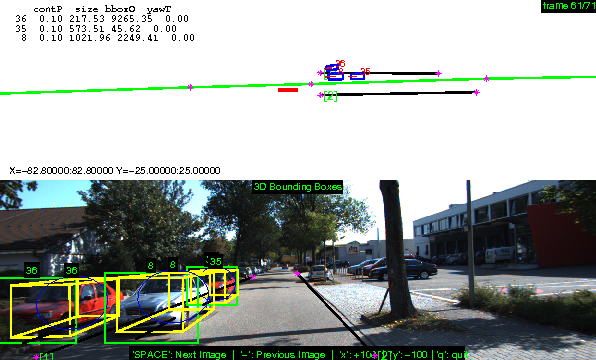
\includegraphics[width=\columnwidth]{results/0009_contPtTracks_size_bboxOcc_yawTstepWiseInference_0000000061.png}
  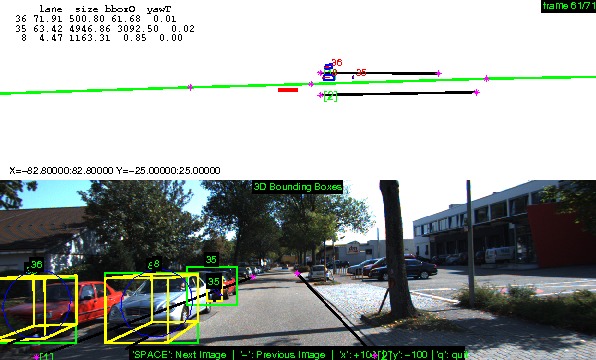
\includegraphics[width=\columnwidth]{results/0009_lane_size_bboxOcc_yawTstepWiseInference_0000000061.png}
  \caption{Qualitative localization results}
  \label{fig:qualLocalizationResults}
\end{figure}


\end{document}
